  
\documentclass[journal,12pt,twocolumn]{IEEEtran}

\usepackage{setspace}
\usepackage{gensymb}
\singlespacing
\usepackage[cmex10]{amsmath}
\usepackage{amssymb}
\usepackage{xurl}
\usepackage{tabularx}
\usepackage{amsthm}
\usepackage{comment}
\usepackage{mathrsfs}
\usepackage{txfonts}
\usepackage{stfloats}
\usepackage{bm}
\usepackage{cite}
\usepackage{cases}
\usepackage{subfig}
\usepackage{arydshln}
\usepackage{longtable}
\usepackage{multirow}

\usepackage{enumitem}
\usepackage{mathtools}
\usepackage{steinmetz}
\usepackage{tikz}
\usepackage{circuitikz}
\usepackage{verbatim}
\usepackage{tfrupee}
\usepackage[breaklinks=true]{hyperref}
\usepackage{graphicx}
\usepackage{tkz-euclide}
\usetikzlibrary{automata, positioning}
\usetikzlibrary{calc,math}
\usepackage{listings}
    \usepackage{color}                                            %%
    \usepackage{array}                                            %%
    \usepackage{longtable}                                        %%
    \usepackage{calc}                                             %%
    \usepackage{multirow}                                         %%
    \usepackage{hhline}                                           %%
    \usepackage{ifthen}                                           %%
    \usepackage{lscape}     
\usepackage{multicol}
\usepackage{chngcntr}
\usepackage{blkarray}

\DeclareMathOperator*{\Res}{Res}

\renewcommand\thesection{\arabic{section}}
\renewcommand\thesubsection{\thesection.\arabic{subsection}}
\renewcommand\thesubsubsection{\thesubsection.\arabic{subsubsection}}

\renewcommand\thesectiondis{\arabic{section}}
\renewcommand\thesubsectiondis{\thesectiondis.\arabic{subsection}}
\renewcommand\thesubsubsectiondis{\thesubsectiondis.\arabic{subsubsection}}


\hyphenation{op-tical net-works semi-conduc-tor}
\def\inputGnumericTable{}                                 %%

\lstset{
%language=C,
frame=single, 
breaklines=true,
columns=fullflexible
}
\begin{document}


\newtheorem{theorem}{Theorem}[section]
\newtheorem{problem}{Problem}
\newtheorem{proposition}{Proposition}[section]
\newtheorem{lemma}{Lemma}[section]
\newtheorem{corollary}[theorem]{Corollary}
\newtheorem{example}{Example}[section]
\newtheorem{definition}[problem]{Definition}

\newcommand{\BEQA}{\begin{eqnarray}}
\newcommand{\EEQA}{\end{eqnarray}}
\newcommand{\define}{\stackrel{\triangle}{=}}
\bibliographystyle{IEEEtran}
\raggedbottom
\setlength{\parindent}{0pt}
\providecommand{\mbf}{\mathbf}
\providecommand{\pr}[1]{\ensuremath{\Pr\left(#1\right)}}
\providecommand{\qfunc}[1]{\ensuremath{Q\left(#1\right)}}
\providecommand{\sbrak}[1]{\ensuremath{{}\left[#1\right]}}
\providecommand{\lsbrak}[1]{\ensuremath{{}\left[#1\right.}}
\providecommand{\rsbrak}[1]{\ensuremath{{}\left.#1\right]}}
\providecommand{\brak}[1]{\ensuremath{\left(#1\right)}}
\providecommand{\lbrak}[1]{\ensuremath{\left(#1\right.}}
\providecommand{\rbrak}[1]{\ensuremath{\left.#1\right)}}
\providecommand{\cbrak}[1]{\ensuremath{\left\{#1\right\}}}
\providecommand{\lcbrak}[1]{\ensuremath{\left\{#1\right.}}
\providecommand{\rcbrak}[1]{\ensuremath{\left.#1\right\}}}
\theoremstyle{remark}
\newtheorem{rem}{Remark}
\newcommand{\sgn}{\mathop{\mathrm{sgn}}}
\providecommand{\abs}[1]{\vert#1\vert}
\providecommand{\res}[1]{\Res\displaylimits_{#1}} 
\providecommand{\norm}[1]{\lVert#1\rVert}
%\providecommand{\norm}[1]{\lVert#1\rVert}
\providecommand{\mtx}[1]{\mathbf{#1}}
\providecommand{\mean}[1]{E[ #1 ]}
\providecommand{\fourier}{\overset{\mathcal{F}}{ \rightleftharpoons}}
%\providecommand{\hilbert}{\overset{\mathcal{H}}{ \rightleftharpoons}}
\providecommand{\system}{\overset{\mathcal{H}}{ \longleftrightarrow}}
	%\newcommand{\solution}[2]{\textbf{Solution:}{#1}}
\newcommand{\solution}{\noindent \textbf{Solution: }}
\newcommand{\cosec}{\,\text{cosec}\,}
\providecommand{\dec}[2]{\ensuremath{\overset{#1}{\underset{#2}{\gtrless}}}}
\newcommand{\myvec}[1]{\ensuremath{\begin{pmatrix}#1\end{pmatrix}}}
\newcommand{\mydet}[1]{\ensuremath{\begin{vmatrix}#1\end{vmatrix}}}
\newcommand*{\permcomb}[4][0mu]{{{}^{#3}\mkern#1#2_{#4}}}
\newcommand*{\perm}[1][-3mu]{\permcomb[#1]{P}}
\newcommand*{\comb}[1][-1mu]{\permcomb[#1]{C}}
\numberwithin{equation}{subsection}
\makeatletter
\@addtoreset{figure}{problem}
\makeatother
\let\StandardTheFigure\thefigure
\let\vec\mathbf
\renewcommand{\thefigure}{\theproblem}
\def\putbox#1#2#3{\makebox[0in][l]{\makebox[#1][l]{}\raisebox{\baselineskip}[0in][0in]{\raisebox{#2}[0in][0in]{#3}}}}
     \def\rightbox#1{\makebox[0in][r]{#1}}
     \def\centbox#1{\makebox[0in]{#1}}
     \def\topbox#1{\raisebox{-\baselineskip}[0in][0in]{#1}}
     \def\midbox#1{\raisebox{-0.5\baselineskip}[0in][0in]{#1}}
\vspace{3cm}
\title{Gate Assignment 1}
\author{Tanay Yadav - AI20BTECH11026}
\maketitle
\newpage
\bigskip
\renewcommand{\thefigure}{\theenumi}
\renewcommand{\thetable}{\theenumi}
Download the python codes from: 
%
\begin{lstlisting}
https://github.com/tanayyadav28/EE3900-Assignments/blob/main/GateAssignment_1/GateAssignment_1.py
\end{lstlisting}
Download the latex-tikz codes from: 
%
\begin{lstlisting}
https://github.com/tanayyadav28/EE3900-Assignments/blob/main/GateAssignment_1/GateAssignment_1.tex
\end{lstlisting}
\section{Problem}
[Gate EC 2015; Q44]
\\For the discrete-time system shown in the figure, the poles of the system transfer function are located at:
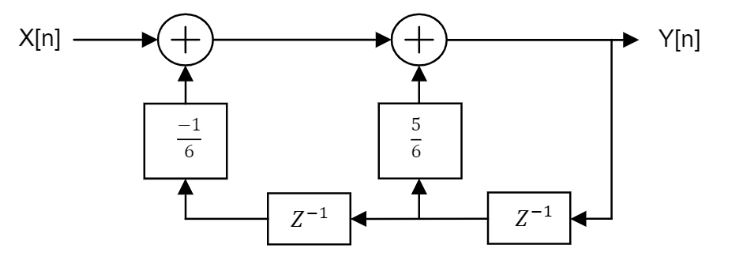
\includegraphics[scale = 0.6]{Q44_img.JPG}
\begin{enumerate}
\setlength\itemsep{0.7em}
    \item $2,3$
    \item $\dfrac{1}{2},3$
    \item $\dfrac{1}{2},\dfrac{1}{3}$
    \item $2,\dfrac{1}{3}$
\end{enumerate}
\section{Solution}
The difference equation of the given discrete-time system is :
\begin{align}
    y[n] &= x[n] - \frac{1}{6}y[n-2] + \frac{5}{6}y[n-1] \\
    \therefore x[n] &= y[n] - \frac{5}{6}y[n-1] + \frac{1}{6}y[n-2] \label{2.0.2}
\end{align}
Applying z-transform to \eqref{2.0.2},
\begin{align}
    X[z] &= Y[z]\left(1 - \frac{5}{6}z^{-1} + \frac{1}{6}z^{-2}\right)
\end{align}
The system transfer function $H(z)$ is given as:
\begin{align}
    H(z) &= \dfrac{Y(z)}{X(z)}\\
    H(z) &= \dfrac{1}{1 - \frac{5}{6}z^{-1} + \frac{1}{6}z^{-2}}\\
    &= \dfrac{z^2}{z^2 - \frac{5}{6}z^{1} + \frac{1}{6}}\\
    &= \dfrac{z^2}{(z-\frac{1}{2})(z-\frac{1}{3})}
\end{align}
The poles can be found by solving the denominator:
\begin{align}
    \left(z-\frac{1}{2}\right)\left(z-\frac{1}{3}\right) &= 0
\end{align}
\\Therefore, the poles of the system transfer function are located at $\frac{1}{2}$ and $\frac{1}{3}$ (Option 3).
\\\\Now, the ROC of $H(z)$ is $\mydet{z} > \frac{1}{2}$.
\\The ROC of $H(z)$ contains the unit circle $\mydet{z} = 1$. Hence, the given system is stable.
\\Considering the difference equation of the given system:
\begin{align}
    x[n] &= y[n] - \frac{5}{6}y[n-1] + \frac{1}{6}y[n-2]
\end{align}
Here, $y[n]$ depends only on the values of the input signal up to and including that time and does not depend on the future values of the input.. Hence, the given system is causal.
\\\\
As the given system is stable and causal, let's find the inverse $z$-transform of $H(z)$ using partial fractions
\begin{align}
    H(z) &= \frac{z^2}{\left(z - \frac{1}{2}\right)\left(z - \frac{1}{3}\right)}\\
    &= \frac{3z}{z - \frac{1}{2}} + \frac{-2z}{z - \frac{1}{3}}
\end{align}
Hence, the impulse response is given as
\begin{align}
    x(n) &= 3\left(\frac{1}{2}\right)^nu(n) - 2\left(\frac{1}{3}\right)^nu(n)
\end{align}
\begin{figure}[h]
    \centering
    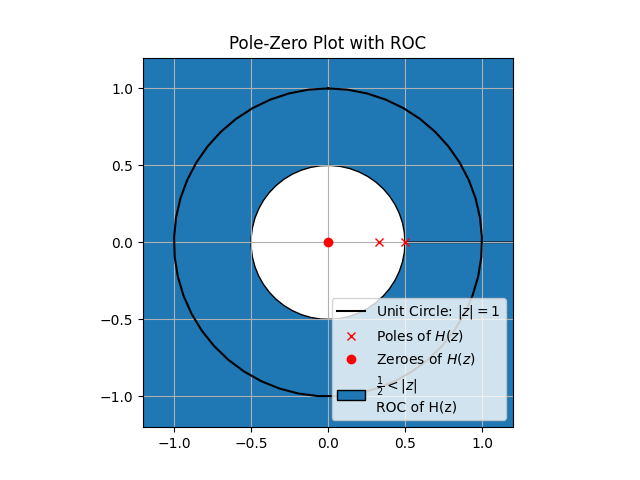
\includegraphics[scale=0.54]{Figure_1.png}
    \label{fig:my_label}
\end{figure}
\end{document}